\chapter{基于Python的硬件开发框架PyHCL}

本章将会介绍用于开发本文所实现的RISC-V微处理器以及SoC平台所使用的基于Python的硬件开发框架PyHCL的技术细节,包括对PyHCL的接口、中间语法树IR、生成器(emitter)以及PyHCL后端生成的FIRRTL语言。在本章的最后会给出PyHCL设计中的创新点以及其如何解决现有硬件开发框架与工具链中固有的问题。

PyHCL的整体设计工具链可以总结如下:开发者使用PyHCL的用户接口在RTL级上对电路逻辑进行描述。为了复用FIRRTL语言作为高层次抽象RTL描述的优势,PyHCL的后端目标生成语言设定为FIRRTL。为了生成FIRRTL代码,PyHCL会根据顶层基于PyHCL接口的电路描述构造中间语法树IR。之后,PyHCL生成器基于语法树生成等效的FIRRTL代码,并将其作为FIRRTL编译器的输入,并将其转化为类网表结构的LoFIRRTL模型,开发者可以在FIRRTL级别上对网表结构进行调整。最后,LoFIRRTL模型转化为可综合的Verilog代码,并可以作为EDA工具的输入进入后端的设计流程。PyHCL设计流程如图2-1所示。

\begin{figure}[htbp]
	\centering
	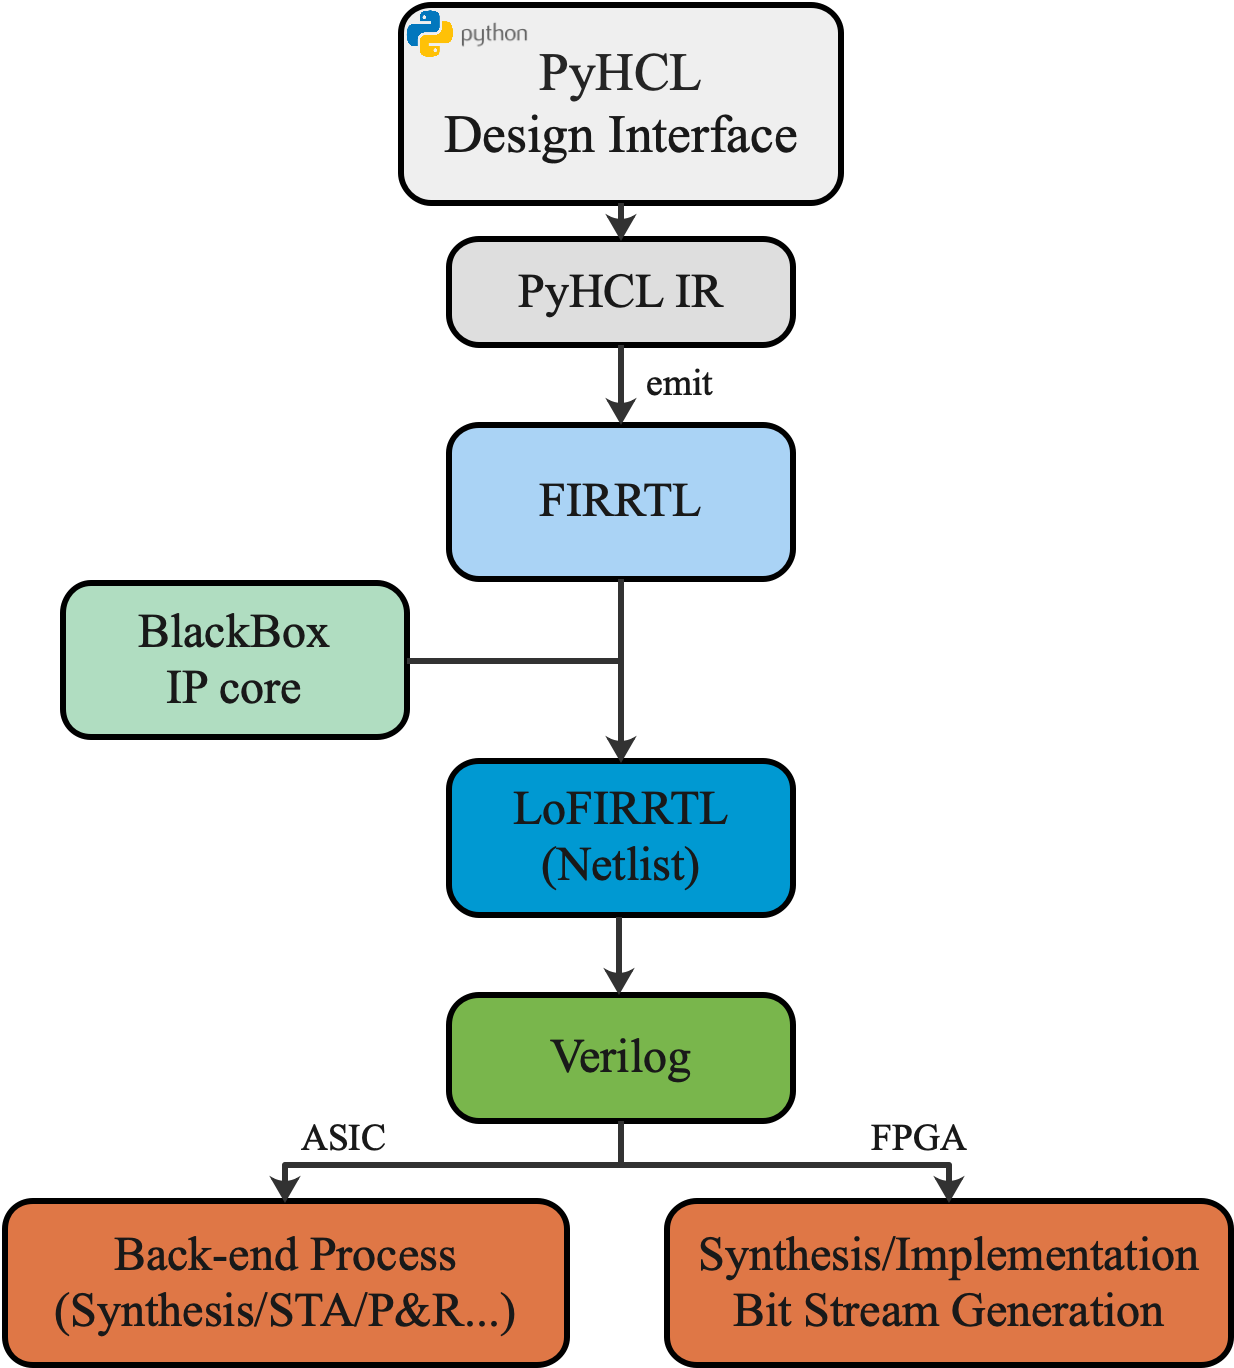
\includegraphics[width=0.95\textwidth]{Photos/PyHCL-Overview.png}
	\caption{PyHCL设计流程}
\end{figure}

\section{PyHCL接口}

PyHCL的设计哲学在于简洁高效的构造(Constructing)电路,而不是单纯的描述(Description)。因此,PyHCL提供了标准的PyHCL数据类型、运算符以及电路元素在RTL级别上构造电路。到目前为止,PyHCL支持三种基本的数据类型:无符号整型(U)、有符号整型(S)以及布尔类型(Bool),其中布尔类型是特殊的无符号类型,在实现时约束为1位的无符号类型来看待。除此之外,PyHCL还支持两种复杂数据类型,分别为向量类型(Vec)以及捆绑类型(Bundle)。向量类型支持对一组相同大小与类型的基本类型数据进行操纵,主要在处理SIMD运算时使用,可以类比为数组。捆绑类型则支持对一组不同大小与类型的基本类型数据进行操作,主要在总线协议接口时使用,可以类比为集合。除此之外,PyHCL还支持隐式的内置时钟类型Clock。通过自定义布尔类型的输入端口,PyHCL支持模块内的多时钟域设计,可以很好的支持异步FIFO[38]等跨时钟域结构的设计。模块内置的隐式或者用户自定义的显式时钟端口可以被模块内部以及外部其他模块引用。

PyHCL运算符通过重载Python内置的运算符来实现。其中最重要的运算符为连接运算符“<<=“,它的作用是驱动右表达式的信号加载到左表达式当中,这涉及到了两个主要的问题:

\begin{enumerate}
	\item 如何匹配Verilog在RTL级描述中的阻塞赋值以及非阻塞赋值。在PyHCL的电路构造过程中,对时序信息是隐含的,对赋值方式的处理在生成Verilog时进行。对于被驱动的电路实体元素,如果是线网类型,则统一使用阻塞赋值。如果是寄存器类型,则统一使用非阻塞赋值。换句话说,开发者在构造电路时不需要考虑赋值类型问题,而只需要关注信号的流动。
	\item 驱动信号与被驱动的电路实体之间的方向关系。PyHCL在构造中间语法树的过程中会对信号的流动方向进行检查,如果发现违例(如模块内部信号连接运算符的左表达式是输入端口),则会抛出异常。
\end{enumerate}

PyHCL接口常用的数据类型及运算符如表2-1所示。

\begin{table}
	\caption{PyHCL常用数据类型及运算符列表}
	\centering
	\small 
	\begin{tabular}{cc}
		\hline 
		PyHCL数据类型 & 用法 \tabularnewline
		\hline 
		\texttt{U} & 无符号整型  \tabularnewline
		\texttt{S} & 有符号整型  \tabularnewline
		\texttt{Bool} & 布尔类型,实现为1位无符号整型  \tabularnewline
		\texttt{Clock} & 隐式内置数据类型,用于表示模块时钟  \tabularnewline
		\texttt{Vec} & 创建一个可索引的包含相同位宽的数据类型的向量结构 \tabularnewline
		\texttt{Bundle}  & 创建一个包含不同位宽的数据类型的集合 \tabularnewline
		\hline
		PyHCL运算符 & 用法 \tabularnewline
		\texttt{<<=} & 连接运算符 \tabularnewline
		\texttt{==}, \texttt{!=} & 逻辑相等,逻辑不等 \tabularnewline
		\texttt{\&}, \texttt{|}, \texttt{\^}, \texttt{\~} & 按位与,按位或,按位异或,按位取反 \tabularnewline
		\texttt{+}, \texttt{-}, \texttt{*}, \texttt{/}, \texttt{\%} & 算术运算符 \tabularnewline
		\texttt{>}, \texttt{>=}, \texttt{<}, \texttt{<=} & 算术比较运算符 \tabularnewline
		\texttt{<<}& 逻辑左移 \tabularnewline
		\texttt{>>} & 逻辑(U)/算术(S)右移,取决于操作数的类型  \tabularnewline
		\texttt{[]} & 位提取运算符,如[5:1]为提取信号第1位到第5位的数据 \tabularnewline
		\hline 
	\end{tabular}
\end{table}

PyHCL接口中提供的电路实体元素是实际电路构造中的功能单元,包括寄存器、线网以及存储单元,它们的PyHCL表示分别为Reg,Wire,以及Mem。所有的PyHCL电路实体元素都预定义在库中,开发者只需要实例化这些电路实体元素就能在设计中使用。PyHCL的电路设计是基于模块化的设计,定义模块的方式通过继承Module基类来实现。为了降低设计者的负担,PyHCL对模块间以及顶层模块与子模块之间的连接提供了自动连接的功能。对于同一层次的两个模块之间的连接,当指定PyHCL进行自动模块连接时,PyHCL在生成语法树时会搜索两个同级模块之间方向相反的IO端口,如果这些端口之间有同样的数据类型、位宽以及名字,或者属于同一个Bundle实体,则PyHCL会将这些IO端口自动连接起来。对于父子节点关系的模块,则需要判断这些端口之间方向相同的IO端口。除此之外,PyHCL的IO端口可以是多级的,在设计总线协议相关的端口时,可以将协议定义的端口作为一个基础的Bundle实体,所有实现了该总线协议接口的模块IO端口都可以包含该Bundle实体。这种多级继承或包含的设计模式与传统的Verilog线性的IO端口声明要更具有鲁棒性。

PyHCL与传统的硬件描述语言的区别在于,PyHCL兼容所有Python的语言特性。所有的PyHCL电路实体元素都可以作为标准的Python内置变量或者实体被解释器所识别。除此之外,PyHCL接口支持多种高级语言特有的设计模式,对于电路设计来说,最具有代表性的两种特性分别是函数式编程以及参数化生成器。

与Verilog中所使用的以变量为中心的设计模式不同,函数式编程以函数为中心,而不是变量,一个函数可以接受其他函数作为参数,也可以返回一个函数对象。这种设计模式更为抽象,且可以将算法以更接近于数学语言的形式表示出来。因此,基于函数式编程的电路设计广泛应用于数字信号处理模块以及外部领域专用的协处理器当中[39]。以一个有限冲激响应(Finite Impulse Response,FIR)滤波器为例子:

\begin{equation}
	y[n]=\sum_{i=0}^N b_i \cdot x[n-i]
\end{equation}

其中N是滤波器的阶数,$b_i$是N阶滤波器在第i时刻($0 \leq i \leq N$)的脉冲响应,$x[n]$是输入信号,$y[n]$是输出信号。在不考虑面积以及性能约束的情况下,这里给出一个对上述滤波器电路实现的PyHCL代码作为例子:

\begin{lstlisting}
	def firFilter(length: int):
		consts = [U(1) for _ in range(length)]
		class FirFilter(Module):
			io = IO(i=Input(U.w(8)), o=Output(U.w(8)))
			taps = [io.i] + [RegInit(U.w(8)(0)) for _ in range(length-1)]
			for a, b in zip(taps, taps[1:]):
				b <<= a
			m = map(lambda x: x[0] * x[1], zip(taps, consts))
			io.o <<= reduce(lambda x, y: x + y, m)
		return FirFilter()
\end{lstlisting}

PyHCL鼓励开发者在电路描述当中使用函数式编程。一个应用函数式编程的典型代码包括两个主要的要素:函数聚合编程以及匿名函数。函数聚合编程表示函数可以作为另一个函数的输入以参数的形式进行传递,抑或是函数作为返回值返回。匿名函数则是临时创建的没有指定名称的函数,匿名函数常常作为函数参数来使用。在上述例子中,PyHCL使用了Python原生的高阶函数来满足上述的两个要素。首先,例子中使用了Python内置的map,zip以及reduce高阶函数来描述乘后加(MAC)运算。两个不同的匿名函数lambda则作为map以及reduce的函数参数来指导对输入信号以及脉冲响应系数的MAC运算。使用函数式编程描述的FIR滤波器更接近于数学语言,将基于Verilog描述中过于繁杂的时序信息隐藏起来,达到快速构建DSP或加速器模块的效果,使构建异构系统变得更有效率。

上述的例子当中除了将函数式编程应用到FIR滤波器的设计当中,还使用了参数化生成器的形式来构造FIR滤波器。可以发现,滤波器的阶数作为函数参数供调用者使用,该函数可以作为一个基础的滤波器生成模版,在其他模块当中进行复用。PyHCL中的参数化生成器中的参数并非是简单的字符串替换,在PyHCL语法树构建以及FIRRTL代码生成过程中参数也作为语法树的一部分,在转换为FIRRTL过程中进行相应的逻辑检查。

总的来说,PyHCL中大范围的函数式编程以及参数化生成器的使用显著的降低了电路设计的迭代周期,以此允许设计者在硬件敏捷设计模式当中应用。

\section{PyHCL IR}

PyHCL IR是介于PyHCL接口以及后端目标FIRRTL语言之间的中间语法树,它由多级的PyHCL IR节点构成。使用PyHCL构造的电路都对应一棵PyHCL语法树。为PyHCL设计介于前后端之间IR语法树的原因在于:

\begin{enumerate}
	\item 在PyHCL前端接口以及后端目标FIRRTL语言之间提供中间语法树可以显著降低PyHCL接口发生更改的风险。在未来,在需要改变接口设计的场合当中,只需要修改接口到中间语法树的对应关系即可。换句话说,PyHCL IR提高了PyHCL开发栈的鲁棒性。
	\item PyHCL IR可以用于进行位宽检查以及数据类型检查。PyHCL IR包含所有电路实体元素在转换为FIRRTL代码所需要的信息,包括数据类型、位宽以及数值。PyHCL IR还可以利用这些信息来调试电路以及抛出设计异常。
	\item PyHCL IR可以在构造语法树的过程中消除冗余的电路结构。如果一个电路实体元素节点没有出现在任何连接运算符的左右子节点,则在生成目标FIRRTL代码的过程中自动去除该节点。
\end{enumerate}

PyHCL IR的节点层级如图2-2所示,该节点图同时也展现了PyHCL多层的设计模式。图2-3展示了一个PyHCL设计时如何使用PyHCL IR节点表示为中间语法树的形式的。

\begin{figure}[htbp]
	\centering
	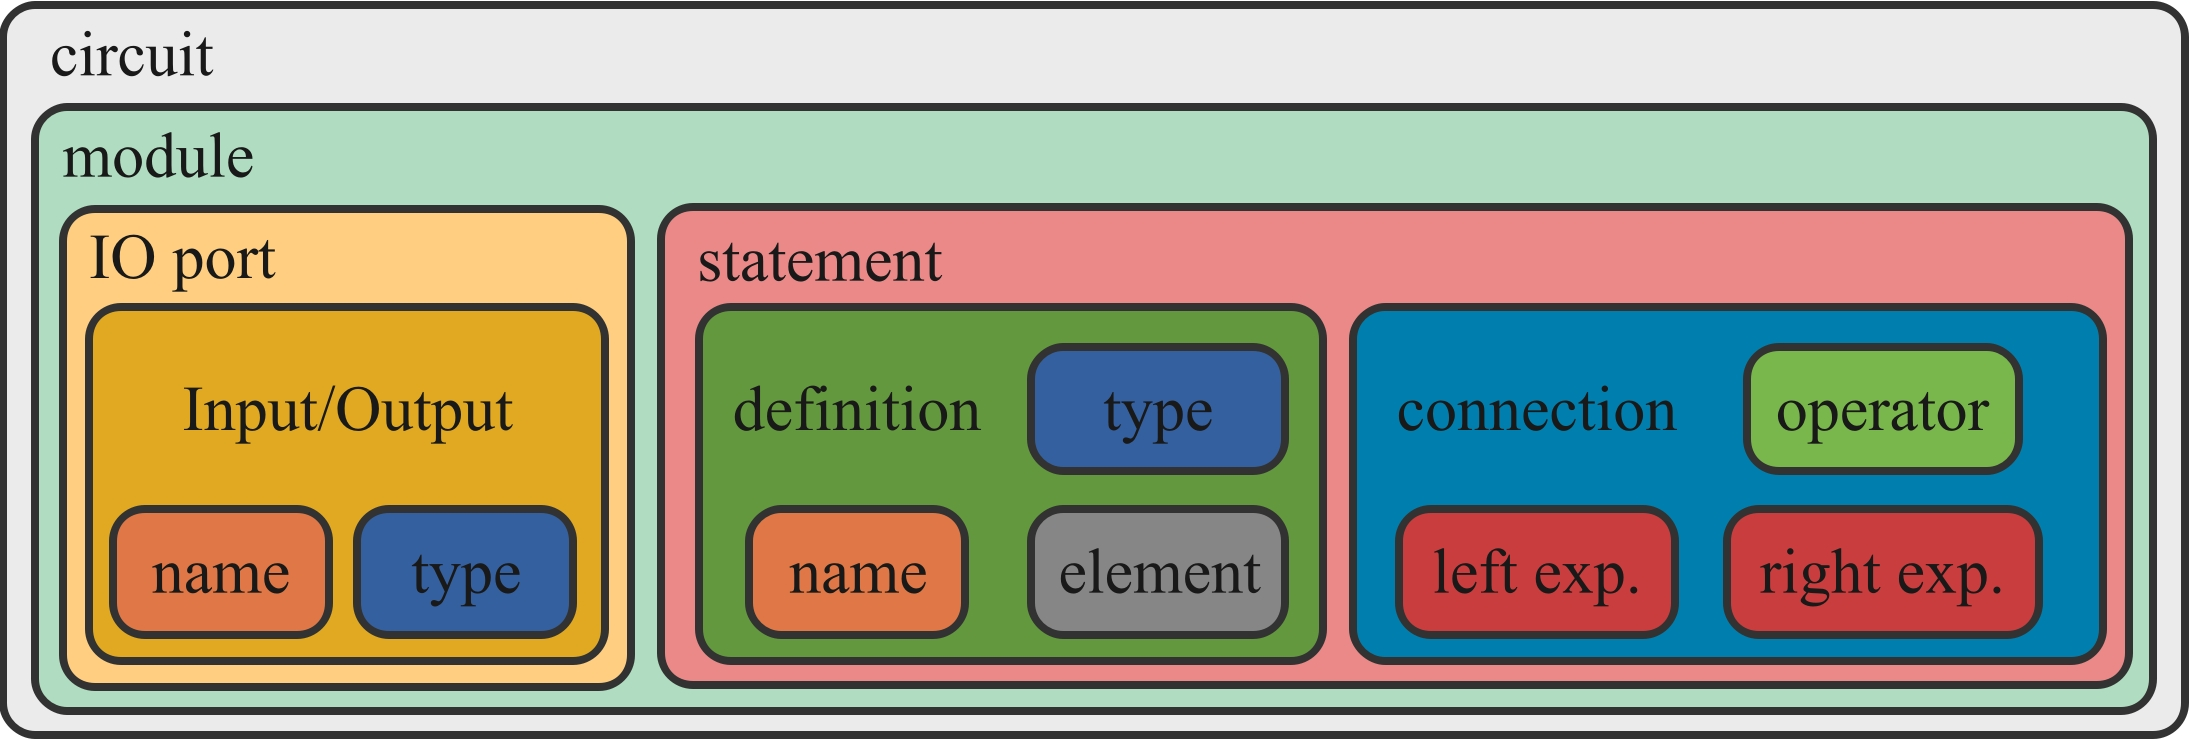
\includegraphics[width=0.95\textwidth]{Photos/PyHCL_IR-Structure.jpg}
	\caption{PyHCL IR的层次化节点设计}
\end{figure}

\begin{figure}[htbp]
	\centering
	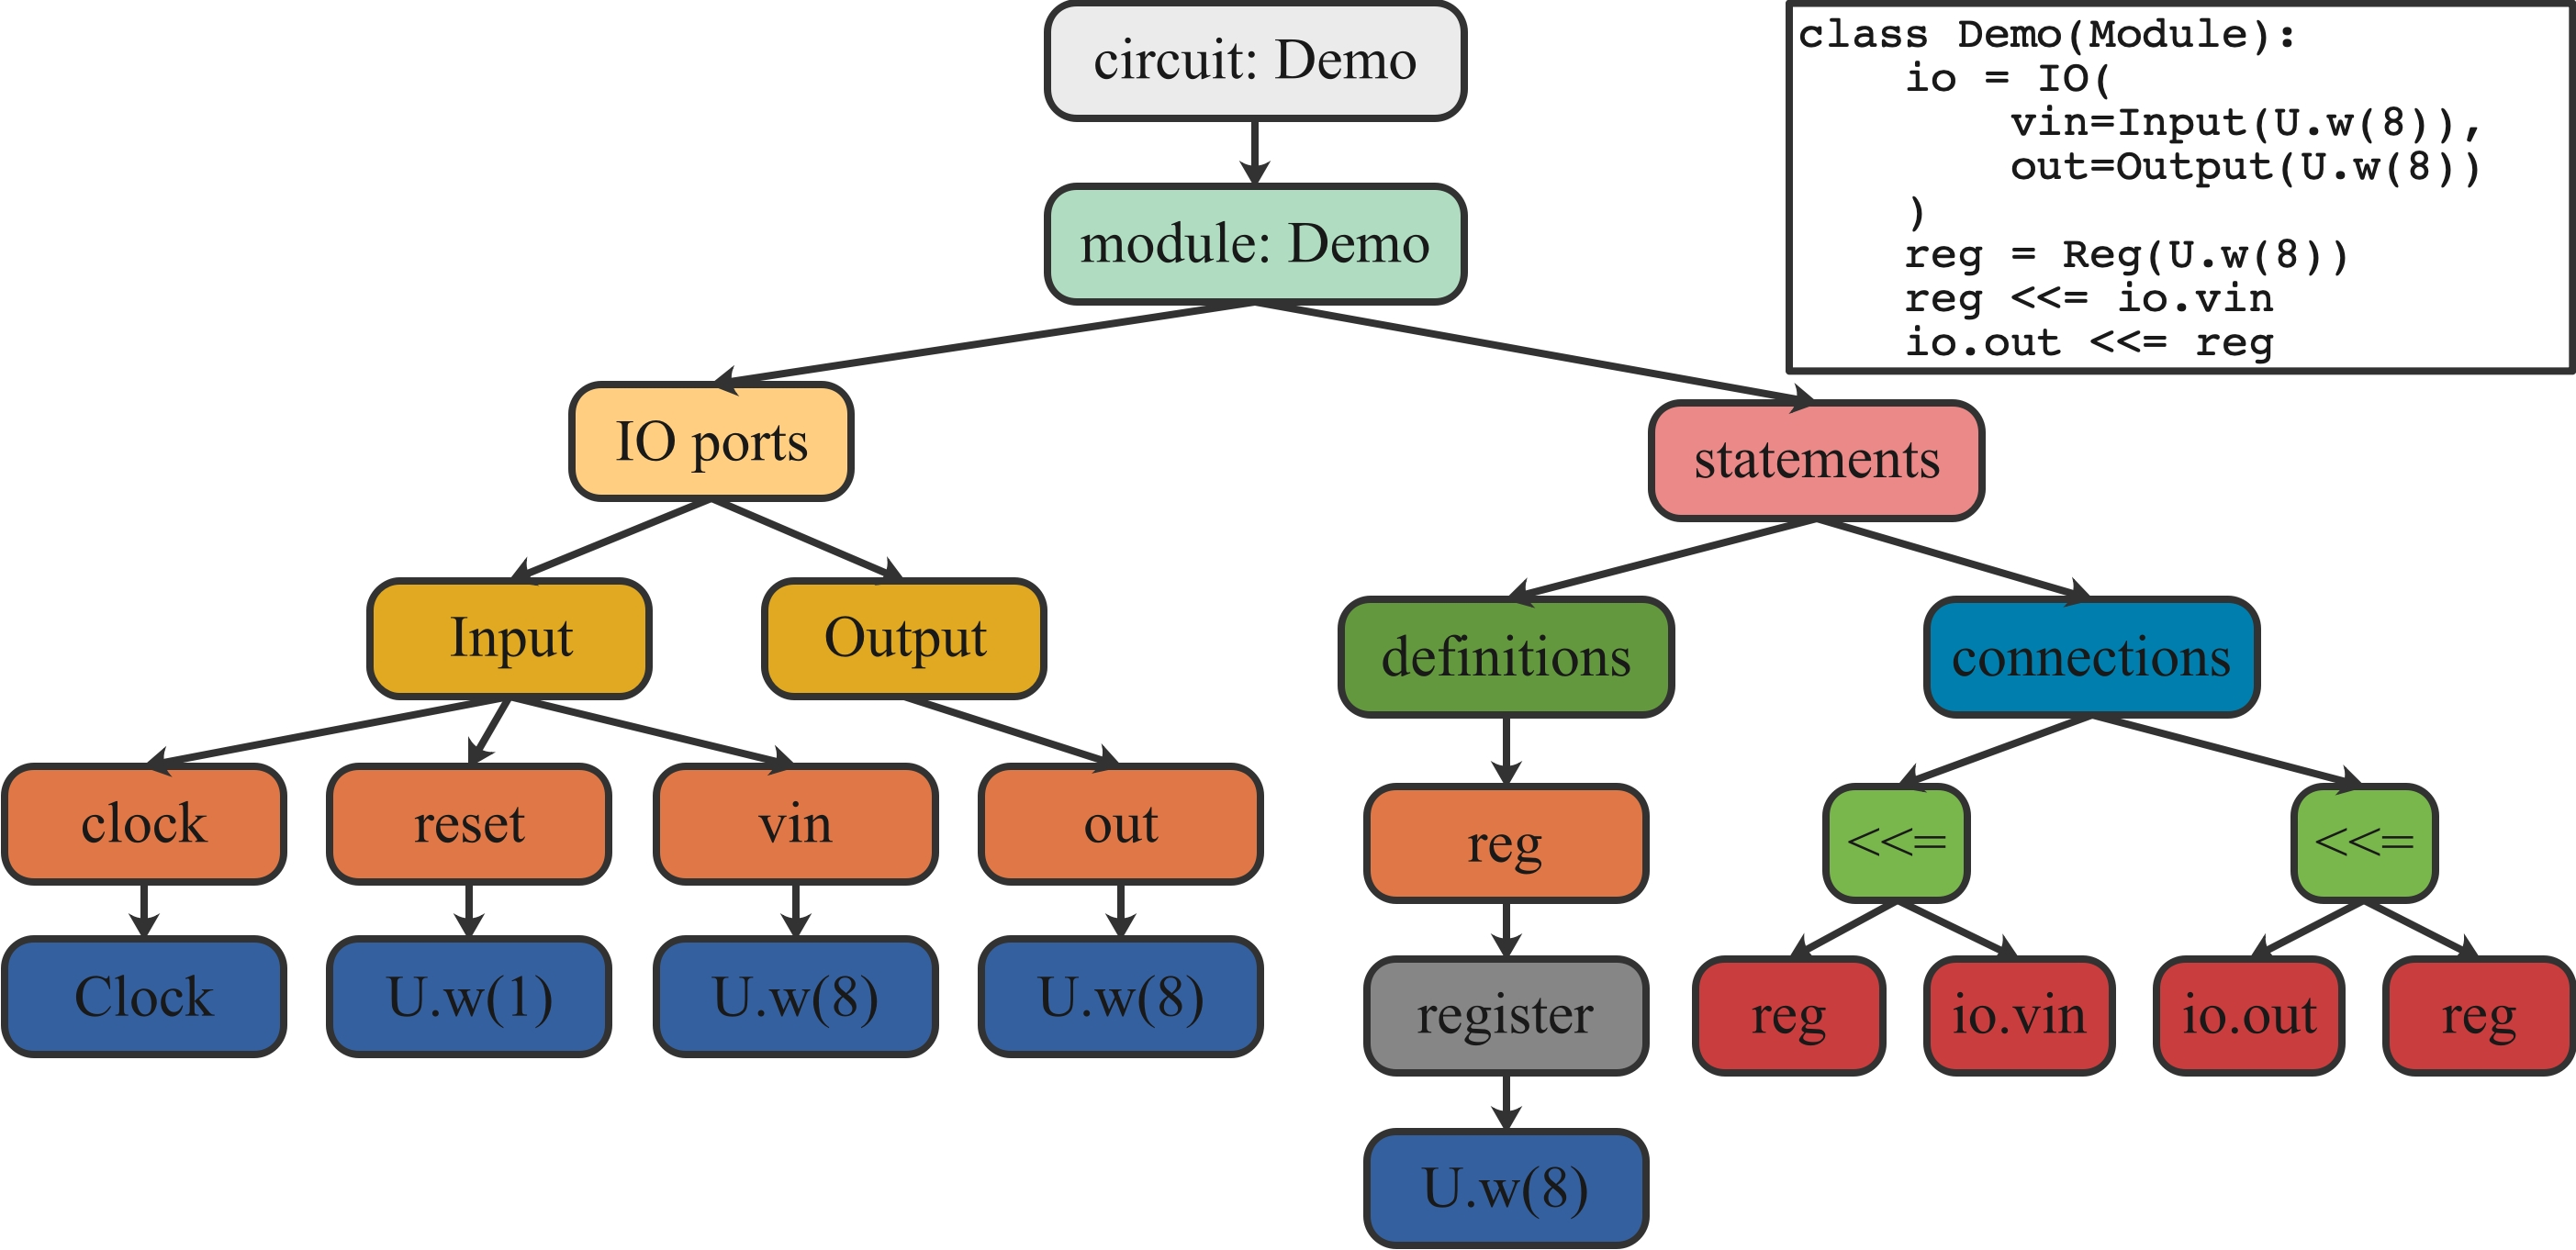
\includegraphics[width=0.95\textwidth]{Photos/PyHCL_IR-Example.jpg}
	\caption{一个PyHCL电路设计使用PyHCL IR节点表示的语法树形式的例子}
\end{figure}

一个典型的PyHCL电路设计通常包含多个PyHCL模块,为了简便起见,图2-3中的例子使用单个模块来作为例子。在多模块的设计当中,顶层模块将同时作为circuit节点。一个PyHCL模块包括两个部分:IO端口以及若干语句块。需要注意的是,PyHCL默认在每个模块构造的过程中自动生成隐式的时钟以及复位端口。PyHCL的语句块包括定义语句以及连接语句。对寄存器、线网以及存储器的定义即为定义语句,同时,在模块内实例化其他模块的语句也是定义语句的一种。对于连接语句来说,PyHCL IR规定连接运算符只能在两个合法的表达式节点之间使用。一个合法的表达式可以是单一的电路实体元素、一个匿名的临时节点(、一个PyHCL内置的工具函数,或者一个返回PyHCL电路实体元素的Python函数。如果一个表达式包含多个运算符,则PyHCL IR会生成多个匿名的临时节点来表示中间结果。PyHCL内置多种提高电路设计效率的工具函数,如Mux以及LookUpTable,其行为与多路选择器的功能类似,且可以接受Python列表或者集合作为输入。在PyHCL中应用函数式编程时,通常会使用高阶函数对寄存器向量或者存储器进行操作,并返回一个PyHCL电路元素实体,如2.1节中的FIR滤波器示例代码中的reduce函数。

从PyHCL代码转换为FIRRTL代码的过程主要是中间语法树生成的过程。PyHCL中负责构造语法树的elaborate函数首先将最顶层的模块作为入口,也就是语法树最顶层的circuit节点,自上而下的构造语法树,而对于以连接运算符为顶层节点的子树,构造的方式则是自底向上进行构造。对于每个模块,首先构造模块对应语法树上的IO端口,一般来说IO端口可以直接将其方向、名字、数据类型以及位宽映射到语法树当中,对于多层级的Bundle IO,则通过递归搜索每个子IO集合的方式来实现。定义语句的构造同样可以直接将电路实体元素类型、名称、数据类型以及位宽映射到语法树当中。对于连接语句,PyHCL通过对连接运算符的左右表达式应用后向搜索算法来构造语法树,如图2-4所示。

\begin{figure}[htbp]
	\centering
	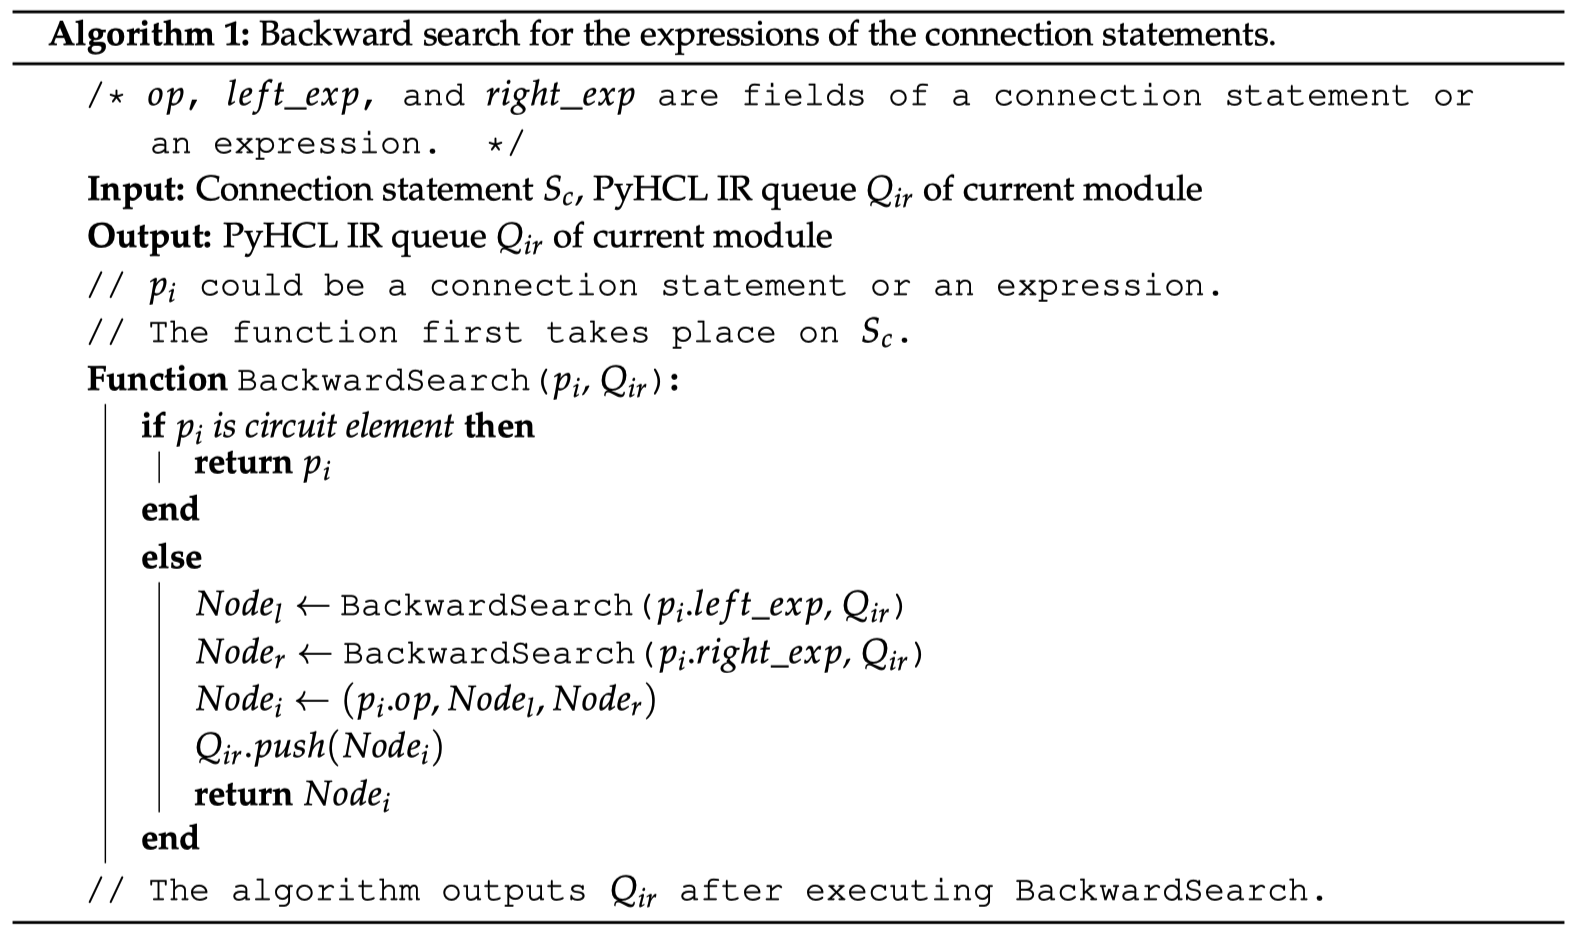
\includegraphics[width=0.95\textwidth]{Photos/back-end_search.png}
	\caption{构造连接语句语法树的后向搜索算法}
\end{figure}

图2-5给出一段连接语句的例子来说明构造PyHCL IR中间语法树的具体过程。

\begin{figure}[htbp]
	\centering
	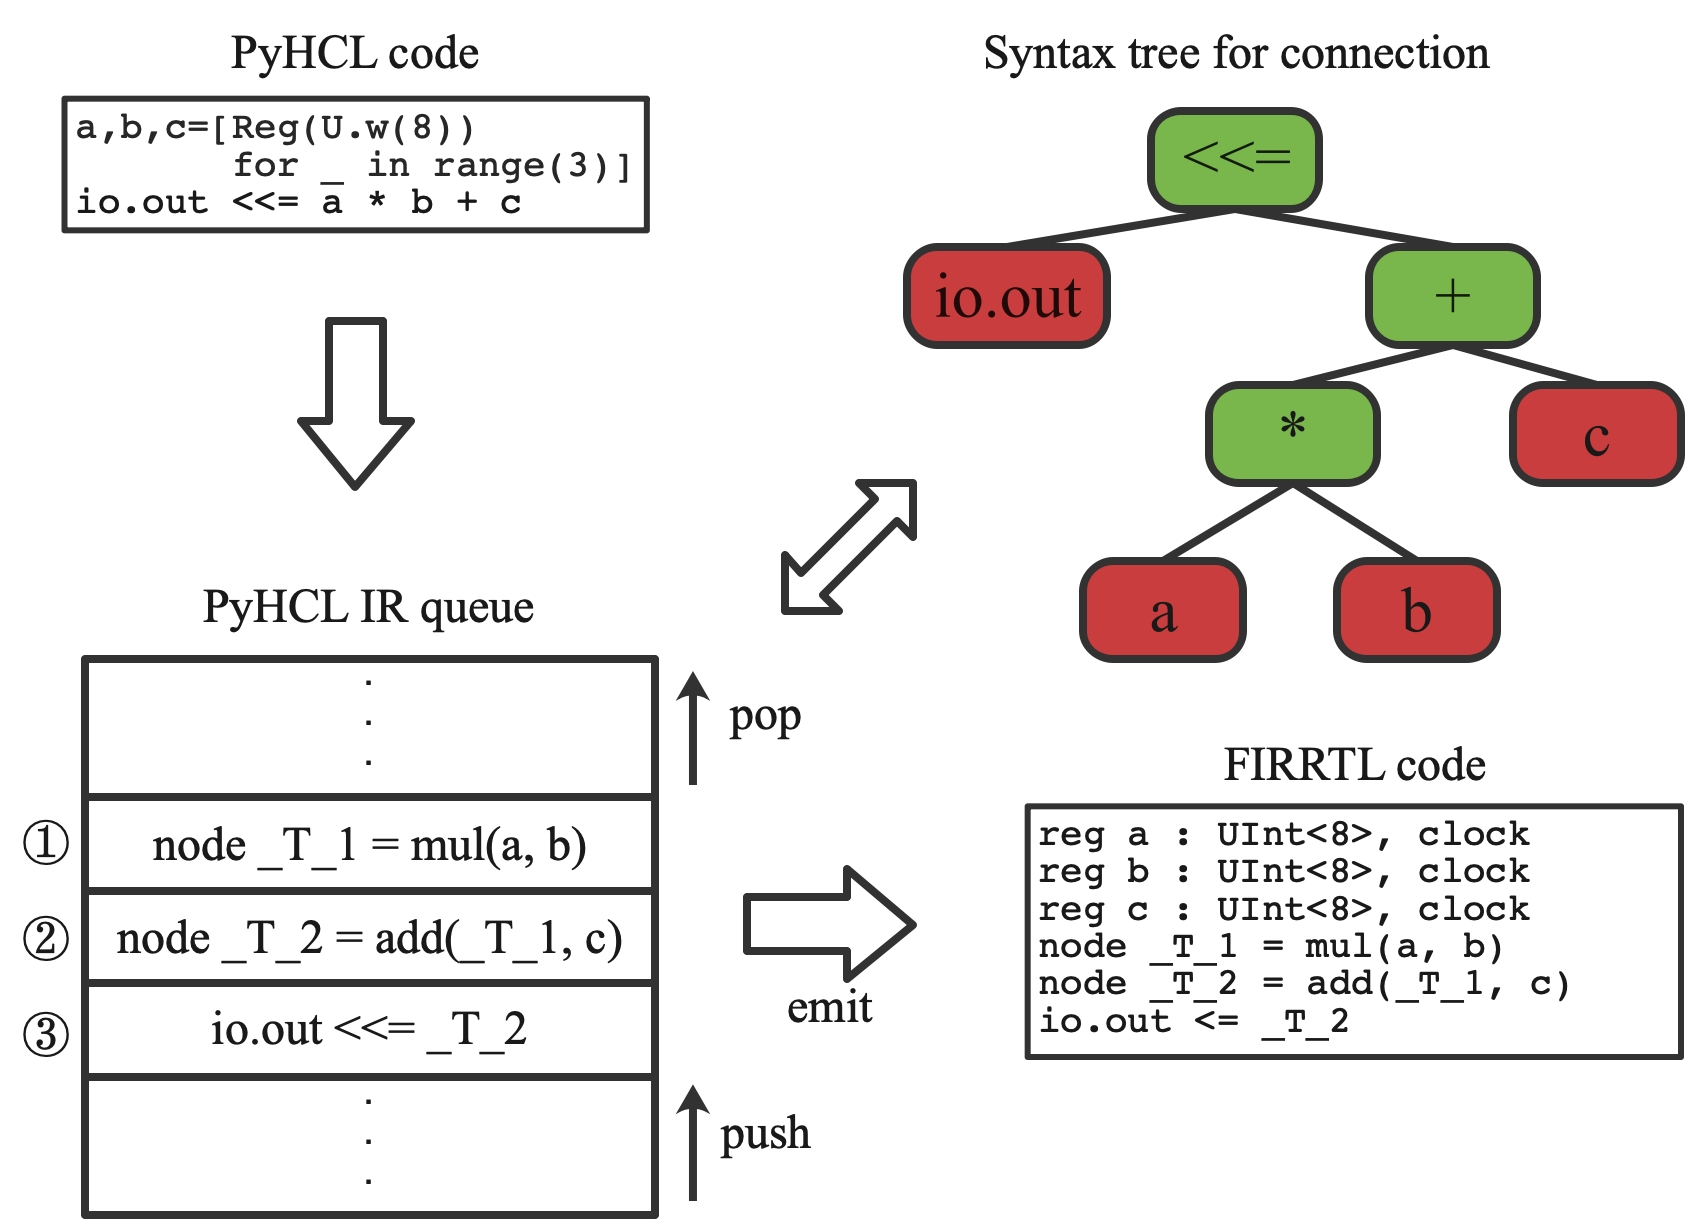
\includegraphics[width=0.95\textwidth]{Photos/Connections-backwared_search.jpg}
	\caption{连接语句的PyHCL IR中间语法树的构造过程}
\end{figure}

PyHCL IR中间语法树在内存中以队列的形式存在,每个PyHCL模块都包含一个PyHCL IR节点的队列。假设一个连接语句$io.out <<= a*b+c$,如图2-5所示。a、b和c都是存储8位无符号数的寄存器,根据运算符的优先级以及图2-4所示的后向搜索算法,语法树的构造过程首先从子表达式$a*b$开始,由于a和b都是叶节点,因此创建一个匿名临时节点$\_T\_1$并压入IR队列当中。接着返回到上一层的调用,对+运算符来说,右表达式寄存器c也是一个叶节点,因此创建第二个匿名临时节点$\_T\_2$,表示$\_T\_1$与c相加的逻辑节点并压入队列中,最后再将连接运算符节点本身压入队列当中。因此对于连接语句的子语法树构造,则是自底向上进行的,其在内存当中的表现形式则是1-3的节点序列,可以发现节点序列实际上就是语法树的前序遍历形式。图2-5中的例子实际上是从2.1节FIR滤波器例子中提取的基本MAC运算逻辑,如果将两个map、reduce高阶函数进行展开,则两个寄存器向量taps以及consts中的每个寄存器都会执行相同的MAC操作:$acc_i <<= taps[i] * consts[i] + acc_{i-1}$。

在构造连接语句的中间语法树过程当中,PyHCL还会进行数据类型检查以及位宽检查与推断的操作。如果左表达式与右表达式的数据类型不一致,则会抛出异常。如果表达式中存在没有显式声明位宽的寄存器或者线网,PyHCL会根据该寄存器或线网参与的连接操作推断其最小合法位宽。如果右表达式驱动的信号位宽大于左表达式的信号位宽,则会抛出异常。需要注意的是,如果一个参数化生成器的可配置参数用于表示位宽信息,则该参数同样会参与到位宽检查与推断的操作当中。这种策略可以将可能的位宽、数据类型违例检查提前进行,而避免电路设计一直到逻辑综合阶段才使用综合器来进行检查。同时,如果一个在定义语句中出现的电路实体元素节点没有出现在任何一个连接语句的左右子树当中,则该节点会被剔除,以此达到消除冗余元素的效果。

在构造当前模块语法树的过程中,如果遇到了子模块的构造声明语句,则会进入对该子模块的递归搜索当中,并返回表示该子模块语法树的队列。在完成了所有模块的语法树构建后,PyHCL生成器会将表示语法树的队列中的节点一一弹出,每个节点都包含有对应的合法FIRRTL语句块,如图2-5所示,并最终生成对应PyHCL电路的FIRRTL代码。

\section{使用FIRRTL构建PyHCL后端}

PyHCL与其他硬件生成框架相比,另一个显著的差异是PyHCL的后端生成目标语言是FIRRTL。大多数现代的硬件生成框架,例如MyHDL与PyRTL,它们的目标生成语言是Verilog,这种HGF称为基于Verilog的HGF。对于基于ASIC后端的集成电路开发流程来说,网表是介于前端RTL级Verilog代码以及后端设计流程(Place \& Route,P\&R)之间的中间表达形式。网表通常在RTL级Verilog代码完成验证工作后通过逻辑综合器生成。网表通常能够保留Verilog代码中的实现细节,换句话说,当Verilog代码能够维持一个相对稳定的电路功能结构时,后端的设计流程就可以更早地介入。如果网表结构在后续的开发迭代流程中发生了重大的改变,那么已经提前完成的后端流程将会浪费掉。基于Verilog的HGF不能够精确的操纵所生成的Verilog代码所表示的电路结构,这是因为这些HGF大都有黑盒制,且这些HGF在进入逻辑综合阶段前都无法地得到网表的任何信息。对于使用基于Verilog的HGF电路设计而言,一些针对原始电路逻辑的细微调整都有可能给生成的Verilog代码结构产生可观的改变,因此这也会导致对网表逻辑结构的改变。因此,使用基于Verilog的HGF进行电路设计,在进入后端P\&R阶段的网表必须保证稳定且尽量不变,否则修改设计所带来的成本将会非常高。

对于PyHCL来说,其后端生成目标语言是FIRRTL,而不是Verilog。FIRRTL具有更接近于网表结构的形式:LoFIRRTL。FIRRTL编译器支持FIRRTL向LoFIRRTL的转化,LoFIRRTL保持了原始FIRRTL的原语但将其转换为更为等效的但更简单、低抽象级别的电路结构。换句话说,LoFIRRTL所表示的电路结构更接近于网表模型。只要PyHCL设计可以保证LoFIRRTL的稳定性,则可以维持该设计所对应的网表结构保持不变。图2-6展示了FIRRTL代码及其对应的LoFIRRTL形式,以及编译后生成的可综合Verilog代码。FIRRTL代码的例子来源于图2-5中的MAC运算。

\begin{figure}[htbp]
	\centering
	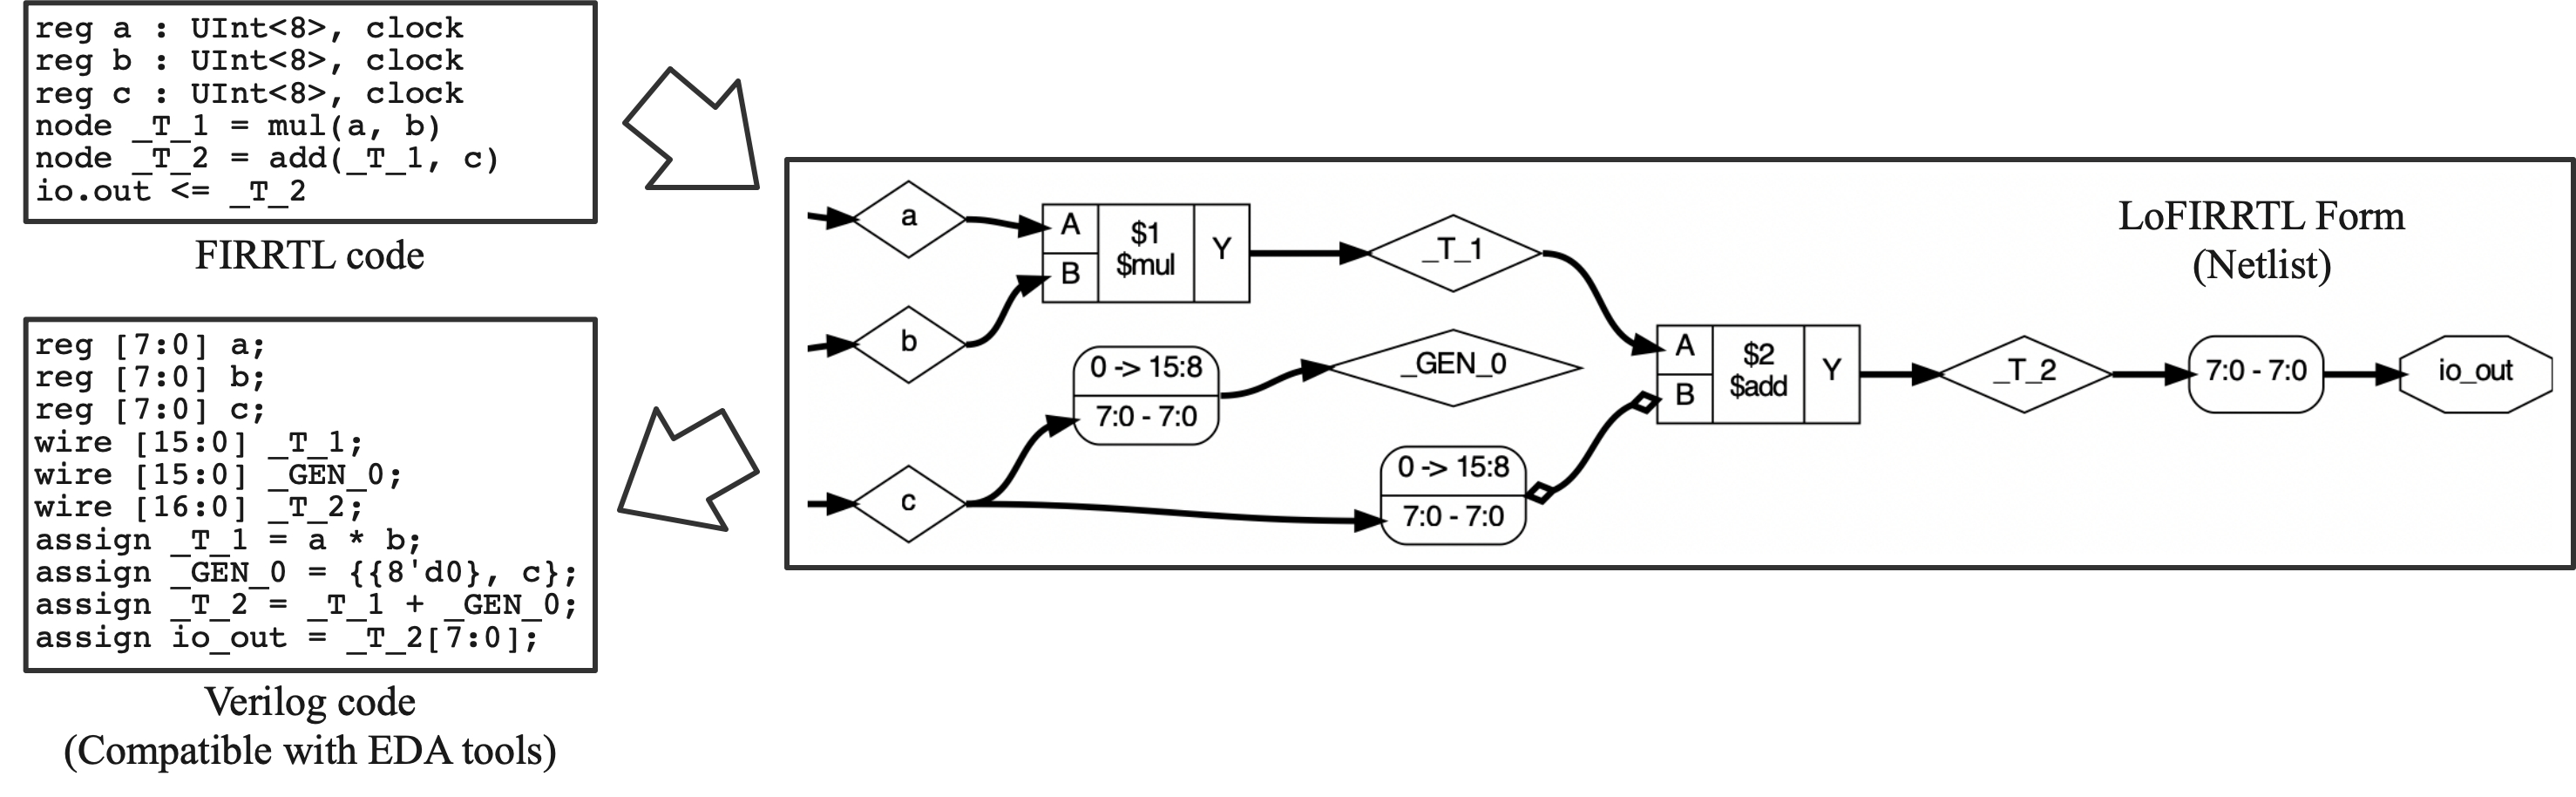
\includegraphics[width=0.95\textwidth]{Photos/FIRRTL_intro.jpg}
	\caption{FIRRTL代码及其对应生成的LoFIRRTL形式、Verilog代码}
\end{figure}

在2.2节提到过,PyHCL中间语法树的IR节点是与FIRRTL原语紧耦合的,这意味着设计者可以通过PyHCL代码精确的控制所生成FIRRTL代码所对应的LoFIRRTL网表结构。因此,使用基于PyHCL进行的硬件设计流程可以将后端P\&R流程尽可能的提前,缩短开发迭代周期,且开发者能够在FIRRTL层级上完成工程改变命令(ECO,Engineering Change Orders)。此时在后续迭代周期中新添加的功能可以通过检查设计所对应的LoFIRRTL网表模型是否有显著改变,来防止浪费上一个迭代周期已完成的后端流程工作。

除此之外,FIRRTL还提供了针对不同FPGA平台宏定义的抽象表达形式,比如不同FPGA平台对平台内置存储器的宏定义。PyHCL设计代码可以通过FIRRTL来保证对包括不同FPGA平台甚至ASIC工艺库的兼容性。综上所述,PyHCL可以显著的缩短硬件开发的迭代周期,并进一步实现硬件敏捷设计的目标。

\section{本章小结}

本章对基于Python的硬件全栈设计框架PyHCL进行的介绍,对PyHCL的接口、中间语法树IR、生成器(emitter)以及PyHCL后端生成的FIRRTL语言进行了介绍。PyHCL通过其独有的函数式编程以及参数化生成器特性,与传统的硬件描述语言以及其他硬件生成框架所区别开来,能够允许用户快速创建电路设计原型并快速迭代,达到硬件敏捷设计的效果。同时,PyHCL的后端FIRRTL语言能够使用户在LoFIRRTL类网表结构上提前进行后端流程,并在LoFIRRTL上完成ECO,以达到加快开发迭代周期的效果。
